\documentclass[11pt,a4paper]{article}
\usepackage[margin=1in]{geometry}
\usepackage{graphicx}
\usepackage{booktabs}
\usepackage{hyperref}
\usepackage{amsmath}
\title{Wine Quality Analysis Report}
\author{Your Name}
\date{\today}

\begin{document}
\maketitle

\section*{Introduction}
This report explores the UCI Wine Quality datasets (red and white)
and presents exploratory plots, a PCA, and regression modeling.

\section{Data Summary}
\begin{itemize}
  \item Total observations: \texttt{r nrow(wine)}
  \item Red vs.\ white counts: see Table~\ref{tab:type_counts}
\end{itemize}

\begin{table}[h]
\centering
\begin{tabular}{lrr}
\toprule
Type & Count \\
\midrule
Red   & 1599 \\
White & 4898 \\
\bottomrule
\end{tabular}
\caption{Counts by wine type}\label{tab:type_counts}
\end{table}

\section{Exploratory Plots}

\begin{figure}[h]
  \centering
  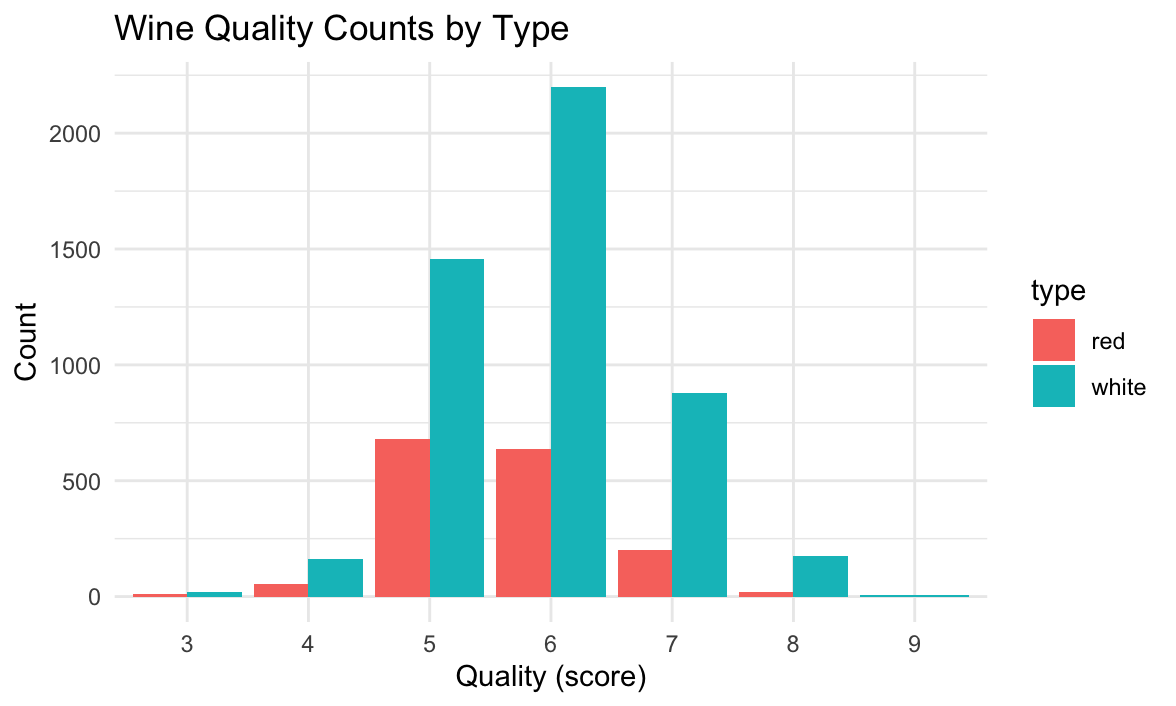
\includegraphics[width=0.8\textwidth]{output/wine-1.png}
  \caption{Wine Quality Counts by Type}
\end{figure}

\begin{figure}[h]
  \centering
  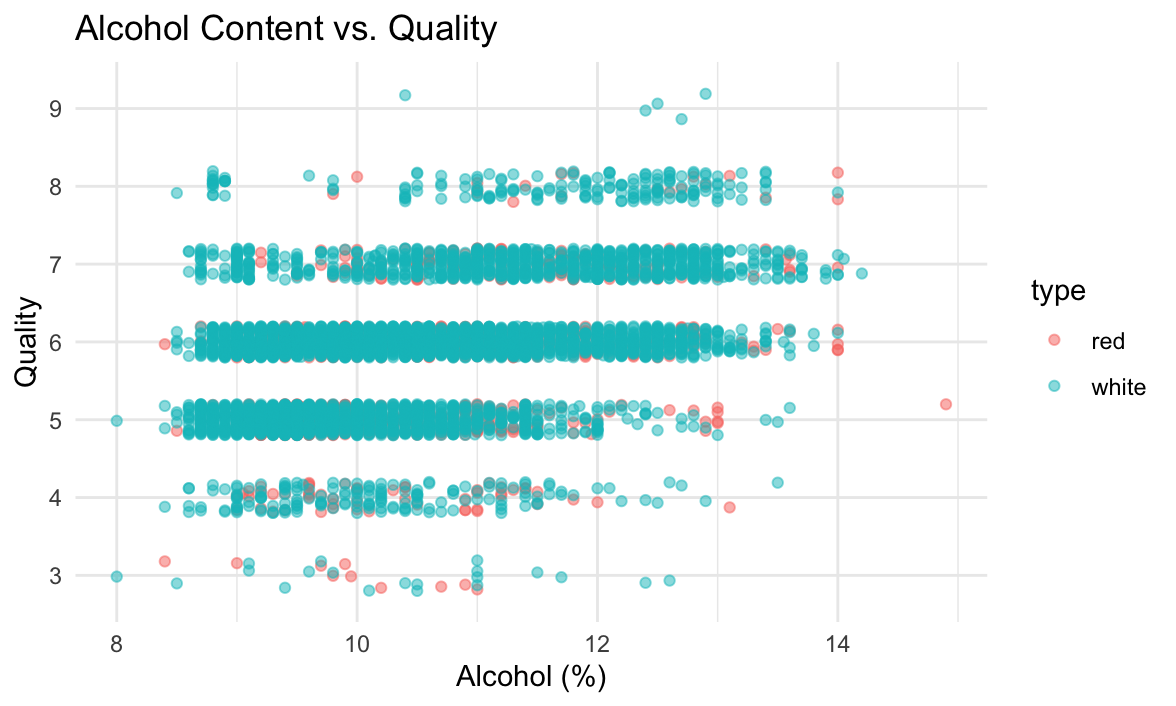
\includegraphics[width=0.8\textwidth]{output/wine-2.png}
  \caption{Alcohol Content vs.\ Quality}
\end{figure}

\section{Correlation Matrix}
\begin{figure}[h]
  \centering
  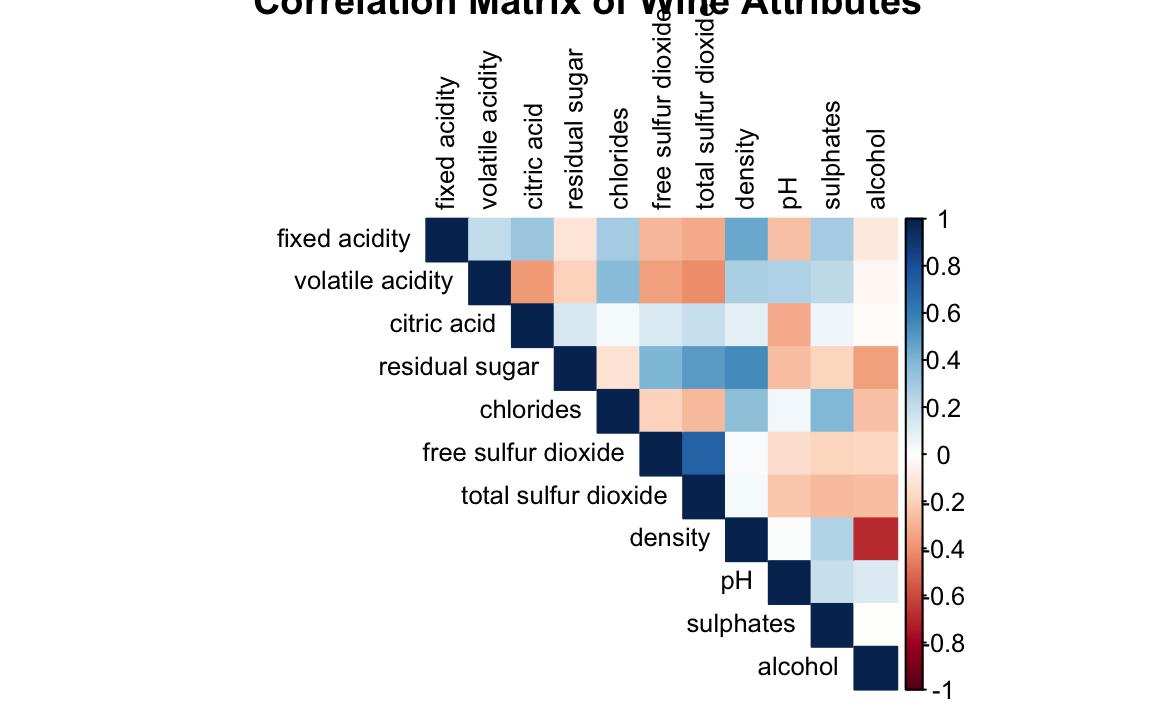
\includegraphics[width=0.7\textwidth]{output/wine-3.png}
  \caption{Correlation Matrix of Numeric Attributes}
\end{figure}

\section{Principal Component Analysis}
\begin{figure}[h]
  \centering
  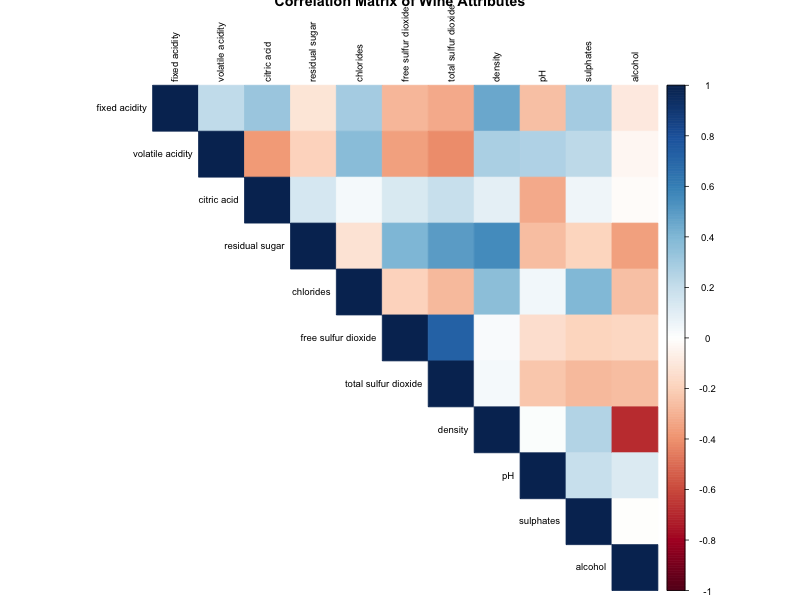
\includegraphics[width=0.7\textwidth]{output/wine-4.png}
  \caption{PCA Scree Plot}
\end{figure}

\begin{figure}[h]
  \centering
  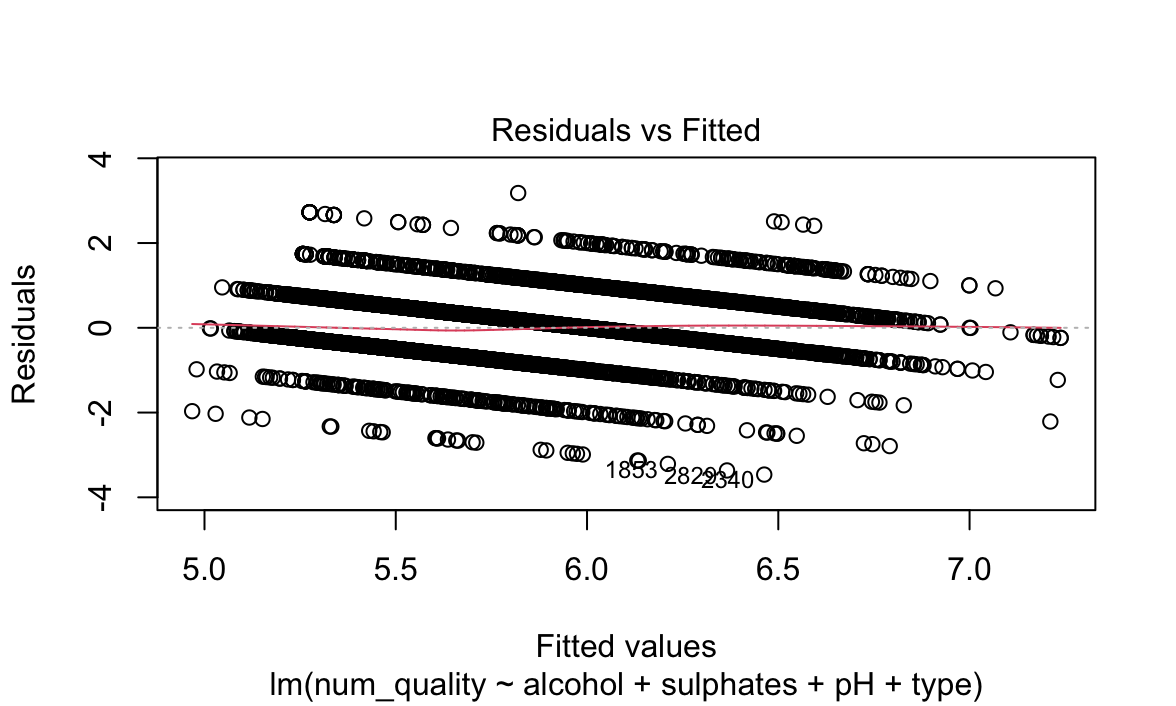
\includegraphics[width=0.7\textwidth]{output/wine-5.png}
  \caption{PCA Biplot}
\end{figure}

\section{Regression Model}
\begin{verbatim}
<<Regression summary printed here>>
\end{verbatim}

\begin{figure}[h]
  \centering
  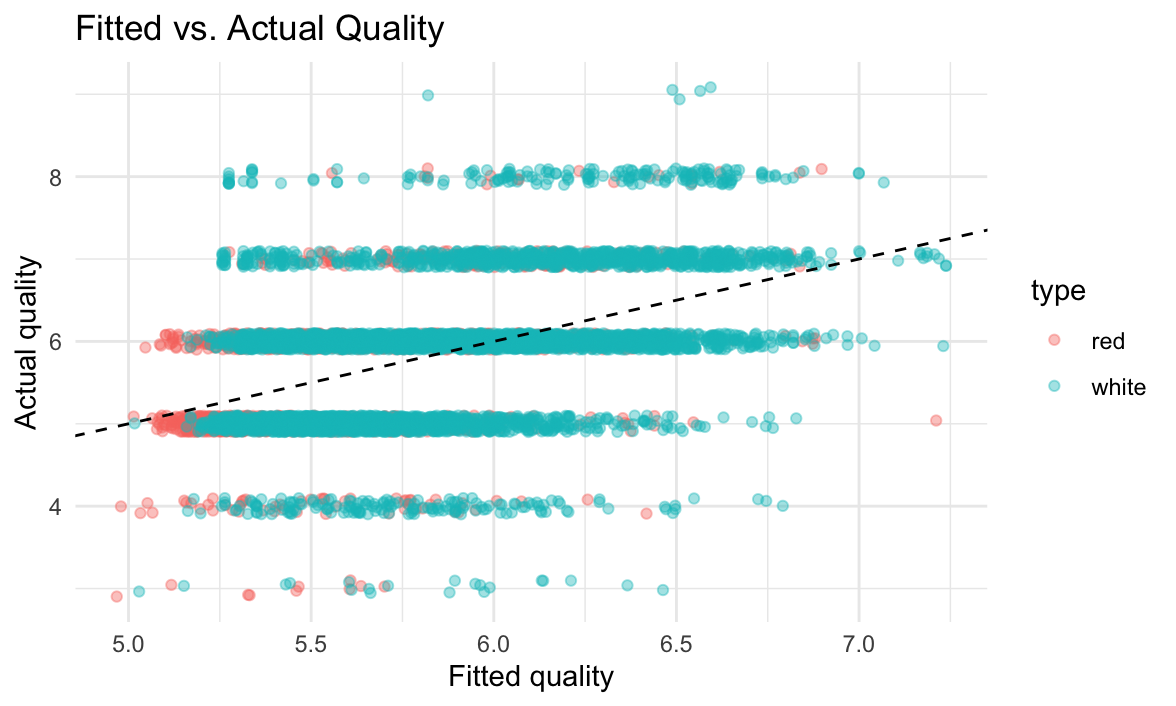
\includegraphics[width=0.8\textwidth]{output/wine-6.png}
  \caption{Fitted vs.\ Actual Quality}
\end{figure}

\section*{Conclusions}
\begin{itemize}
  \item White wines tend to score slightly higher than red.  
  \item Alcohol, sulphates, and pH were significant predictors of quality.  
  \item PCA shows that the first two components capture most variance.  
\end{itemize}

\end{document}
